% Please use the skeleton file you have received in the 
% invitation-to-submit email, where your data are already
% filled in. Otherwise please make sure you insert your 
% data according to the instructions in PoSauthmanual.pdf

% JRP added to avoid ifpdf name clash in TexShop
\RequirePackage{ifpdf}
%%% END JRP

\documentclass{PoS}

%JRP added
%Uncomment next line if AMS fonts required
 \usepackage{graphicx}
 \usepackage{epstopdf}

 %%% END JRP

\title{Cosmology from EoR/Cosmic Dawn}

\ShortTitle{EoR/CD Cosmology}

\author{\speaker{Pritchard}\thanks{A footnote may follow.}, Ichiki, Mesinger, Metcalf, Santos, Chang, Furlanetto, Choudhury, Zaroubi, Chen, Weller, Abdalla,  on behalf of the Cosmology-SWG and EoR/CD-SWG\\
        Imperial College London\\
        E-mail: \email{j.pritchard@imperial.ac.uk}}
        
\author{Robert Benton Metcalf\\
        Dipartimento di Fisica e Astronomia, Universit\'{a} di Bologna, viale B. Pichat 6/2 , 40127, Bologna, Italy\\
        E-mail: \email{robertbenton.metcalf@unibo.it}}

\author{Alkistis Pourtsidou\\
        Dipartimento di Fisica e Astronomia, Universit\'{a} di Bologna, viale B. Pichat 6/2 , 40127, Bologna, Italy\\
        E-mail: \email{alkistis.pourtsidou@unibo.it}}

%\author{Another Author\\
%        Affiliation\\
%        E-mail: \email{...}}

\abstract{SKA Phase 1 will build upon early detections of the EoR by precursor instruments, such as MWA, PAPER, LOFAR, and HERA, to make the first high signal-to-noise measurements of fluctuations in the 21 cm brightness temperature from both reionization and the cosmic dawn. This will allow both imaging and statistical maps of the 21cm signal at redshifts $z=6-30$ and constrain the underlying cosmology and evolution of the density field. This era includes nearly 60\% of the (in principle) observable volume of the Universe and many more linear modes than the CMB, presenting an opportunity for SKA to usher in a new level of precision cosmology. This optimistic picture is complicated by the need to understand and remove the effect of astrophysics, so that systematics rather than statistics will limit constraints.

This chapter will describe the cosmological, as opposed to astrophysical, information available to SKA Phase 1. Key areas for discussion include: cosmological parameters constraints using 21cm fluctuations as a tracer of the density field; lensing of the 21cm signal, constraints on heating via exotic physics such as decaying or annihilating dark matter; impact of fundamental physics such as non-Gaussianity or warm dark matter on the source population; and constraints on the bulk flows arising from the decoupling of baryons and photons at $z=1000$. The chapter will explore the path to separating cosmology from `gastrophysics', for example via velocity space distortions and separation in redshift. We will discuss new opportunities for extracting cosmology made possible by the sensitivity of SKA-1 and explore the advances achievable with SKA-2.
}

\FullConference{
Advancing Astrophysics with the Square Kilometre Array\\
June 8-13, 2014\\
Giardini Naxos, Italy}

%Add new definitions here
%user defined shortcuts
%Journal definitions
\newcommand{\apj}{ApJ}
\newcommand{\apjl}{ApJ}
\newcommand{\apjs}{ApJS}
\newcommand{\aap}{A \& A}
\newcommand{\aj}{AJ}
\newcommand{\araa}{ARAA}
\newcommand{\mnras}{MNRAS}
\newcommand{\physrep}{Phys. Rep.}
\newcommand{\prd}{PRD}
\newcommand{\nat}{Nat.}
\newcommand{\jcap}{JCAP}
\newcommand{\sovast}{Sov. Astron.}
\newcommand{\nar}{New Astron. Rev.}
\newcommand{\apss}{Astrophys. \& Space. Sci.}
\newcommand{\aapr}{A \& A Rev.}

\newcommand{\ud}{{\rm d}}

%%%% END NEW DEFINITIONS

\begin{document}

%%%%%%%%%%%%%%%%%%%%%%%%%%%%%
%%%%%%%%%%%%%%%%%%%%%%%%%%%%%
\section{Introduction}

The years since the COBE observations of the CMB have ushered in an age of precision cosmology. Key cosmological parameters have been made possible by measurements of the distribution of matter in the Universe through WMAP and Planck observations of CMB anisotropies and large volume galaxy surveys such as SDSS. These surveys have made precision measurements of parameters describing the matter content of the Universe - the baryons $\Omega_b$, dark matter $\Omega_c$, dark energy $\Omega_\Lambda$, radiation $\Omega_r$, and neutrinos $\Omega_\nu$ - and the physics of inflation - via the tilt $n_s$, amplitude $A_s$, running $\ud n_s/\ud\log k$ or the primordial potential power spectrum and $r$ the ratio of tensor-to-scalar modes produced by inflation. These measurements have firmly established the basic picture of our Universe, known widely as the $\Lambda$CDM model of cosmology.

Despite this progress, measuring these numbers is only the first step towards a deep understanding of the underlying physics. Our ignorance of the nature of the dark matter and the dark energy or how neutrinos acquire mass and what value that mass takes are just two questions that modern cosmology hopes to address. Over the next decade two paths will help shed light on this. The simplest is simply to measure these cosmological parameters ever more precisely and over a wider range of times and scales in the hope of gaining further insights. The exemplar of this is with dark energy, where attempts to measure the redshift evolution of the dark energy density, parameterised by an equation of state $w(z)$, might distinguish a true cosmological constant from more general dark energy or modified gravity. For others there are critical thresholds of precision required to distinguish physical scenarios - for example, measuring the sum of the neutrino masses $M_\nu\lesssim0.1$ would determine the neutrino mass hierarchy. Clearly more precision is a good thing, but it is not the only path forward.

Secondly, we can seek signatures of new physics in ways distinct from the distribution of large scale matter. The processes that produce dark matter will also allow it to annihilate and maybe to decay. The release of energy might have impact on the surrounding environment, heating the intergalactic medium. Pursuing unique signatures of new physics in new regimes will be a key part of the next decade.

The SKA is uniquely placed to probe cosmology as it is capable of mapping the Universe over wide volumes and an unprecedented range of redshifts. Figure \ref{fig:volume} illustrates the additional range of volume and redshifts that the SKA will constrain. In this chapter, we will focus on the new opportunities created by SKA observations of the epoch of reionization (EoR) and the cosmic dawn (CD). This period has never before been observed offering a unique opportunity to test the consistency of the $\Lambda$CDM model and search for new hints to the great unanswered questions of cosmology.

\begin{figure}[htbp]
\begin{center}
\includegraphics[scale=0.6]{figures/plotcircles.png}
\caption{Illustration of the volume probed by SKA}
\label{fig:volume}
\end{center}
\end{figure}

\cite{furlanetto2006dm}

%%%%%%%%%%%%%%%%%%%%%%%%%%%%%
%%%%%%%%%%%%%%%%%%%%%%%%%%%%%
\section{Cosmological parameters from density fluctuations}

{\bf Introduce fisher matrix formalism}

In this section, we explore the ability of SKA to constrain cosmological parameters via observations of the density field. Just as galaxy surveys constrain cosmology by using galaxies as a tracer of the linear density field, SKA can constrain cosmology by using the 21 cm brightness temperature as a tracer of the density field. This is not an unproblematic assertion, since brightness temperature fluctuations may be sourced by variation in the spin temperature and neutral fraction in addition to the density field. 

\begin{equation}\label{deltatb}
\delta T_B=(1+\delta)x_H...
\end{equation}
Equation \ref{deltatb} shows how these different terms come into play. In a regime where $T_S\gg T_{\rm CMB}$ and $x_H=1$ then $\delta T_B$ will be an unbiased tracer of the density field. At all other times the effects of astrophysics must be modelled and removed or somehow avoided. We will return to a discussion of this point in \S\ref{sec:separation} as this is a critical point.

In this section, we take the optimistic view that there will a regime in which $\delta T_b\propto(1+\delta)$ so that the 21cm signal provides a clean measurement of the density field. This approach enables us to evaluate the best case scenario for SKA in measuring cosmological parameters. By comparing this to galaxy surveys we get a sense of how competitive SKA could be, if astrophysics could be overcome.

The sensitivity of a radio interferometer to the 21cm power spectrum has been well studied \cite{bowman2005, mcquinn2006,mao20??} and we follow the same approach here. The variance of a 21 cm power spectrum estimate for a single
$\mathbf{k}$-mode with line of sight component $k_{||}=\mu k$ is given by
\cite{lidz2007}:
\begin{equation}
\sigma_P^2(k,\mu)= \frac{1}{N_{\rm field}}\left[\bar{T}_b^2P_{21}(k,\mu)+T_{\rm sys}^2\frac{1}{B t_{\rm int}}\frac{D^2\Delta D}{n(k_\perp)}\left(\frac{\lambda^2}{A_e}\right)^2\right]^2.
\end{equation}

The first term on the right-hand-side
of the above expression provides the contribution from sample variance,
while the second describes the thermal noise of the radio telescope.  The
thermal noise depends upon the system temperature $T_{\rm sys}$, the survey
bandwidth $B$, the total observing time $t_{\rm int}$, the conformal
distance $D(z)$ to the center of the survey at redshift $z$, the depth of
the survey $\Delta D$, the observed wavelength $\lambda$, and the effective
collecting area of each antennae tile $A_e$.  The effect of the
configuration of the antennae is encoded in the number density of baselines
$n_\perp(k)$ that observe a mode with transverse wavenumber $k_\perp$
\cite{mcquinn2005}.  Observing a number of fields $N_{\rm field}$ further reduces the variance.

Estimates of the error on a power spectrum measurement are calculated using the Fisher matrix formalism, so that the $1-\sigma$ errors on the model parameter $\lambda_i$ are $(\mathbf{F}_{ij}^{-1})^{1/2}$, where 
\begin{equation}
F_{ij}=\sum_{\rm \mu} \frac{\epsilon k^3 V_{\rm survey}}{4\pi^2}\frac{1}{\sigma_P^2(k,\mu)}\frac{\partial P_{T_b}}{\partial \lambda_i}\frac{\partial P_{T_b}}{\partial \lambda_j}.
\end{equation}
In this equation, $V_{\rm survey}=D^2\Delta D(\lambda^2/A_e)$ denotes the
effective survey volume of our radio telescopes and we assume wavenumber
bins of width $\Delta k=\epsilon k$.  We will be interested in the cases
where $\lambda_i=\{\bar{P}_{T_b}\}$ and $\lambda_i=\{
P_{\mu^0},\,P_{\mu^2},\,P_{\mu^4}\}$.

{\bf sensitivity plot for various experiments relative to density field}

\begin{table}[htdp]
\caption{Low-frequency radio telescopes and their parameters.  We specify the number of antennae $N_a$, total collecting area $A_{\rm tot}$, bandwidth $B$, and total integration time $t_{\rm int}$ for each instrument. These values are fixed at $z=??$ and extrapolated to other frequencies using $A_{\rm tot}=N_{\rm ant}N_{\rm dip}A_{\rm dip}$ with the number of antennae per station $N_{\rm dip}=289$ and $A_{\rm dip}=\min(\lambda^2/3,3.2\,{ \rm m^2})$.}
\begin{center}
\begin{tabular}{ccccccc}
\hline
\hline
Array & $N_a$ & $A_{\rm tot}(10^3\,{\rm m^2})$ & $B$ (MHz) & $t_{\rm int}$ (hr)& $R_{\rm min} (m)$ & $R_{\rm max} (km)$\\
\hline
MWA & 112 & 1.6  & 8 & 1000 & 4 & 0.75\\
LOFAR Core & 48 & 38.6  & 8 & 1000 & 100 & 1.5\\
HERA & 331 & 50.0  & 8 & 1000 & 14.3 & 0.3\\
SKA0 & 850$\times$0.5 & 290$\times$0.5  & 8 & 1000 & 35 & 2\\
SKA1 & 850 & 290  & 8 & 1000 & 35 & 2\\
SKA2 & 850$\times$4 & 290$\times$4 & 8 & 1000 & 35 & 2\\
\hline
\hline
\end{tabular}
\end{center}
\label{tab:telescopes}
\end{table}%

We first illustrate the sensitivity of different iterations of SKA in Figure \ref{fig:sensitivity}, where we take the parameters in Table \ref{tab:telescopes} for SKA0 - with 50\% of the SKA1 baseline collecting area, SKA1, and SKA2 - with x4 the collecting area of SKA1. For each of these we assume a filled core followed by $r^{-2}$ distribution out to a maximum radius $R_{\max}$. HERA is assumed to have a uniform antennae distribution.

{\bf SKA1 has 911 stations total with 899 in the core and 650 stations within a radius of 1km accounting for ~75\% of the total number of stations and collecting area. Physical station size is 35m. Stations have 289 antennae with antennae area $A_e=\lambda^2/3$ giving $3.2m^2$ at 110MHz. At lower frequencies the array is densely packed and has constant collecting area, at higher frequencies the array becomes sparse.}

\begin{figure}[htbp]
\begin{center}
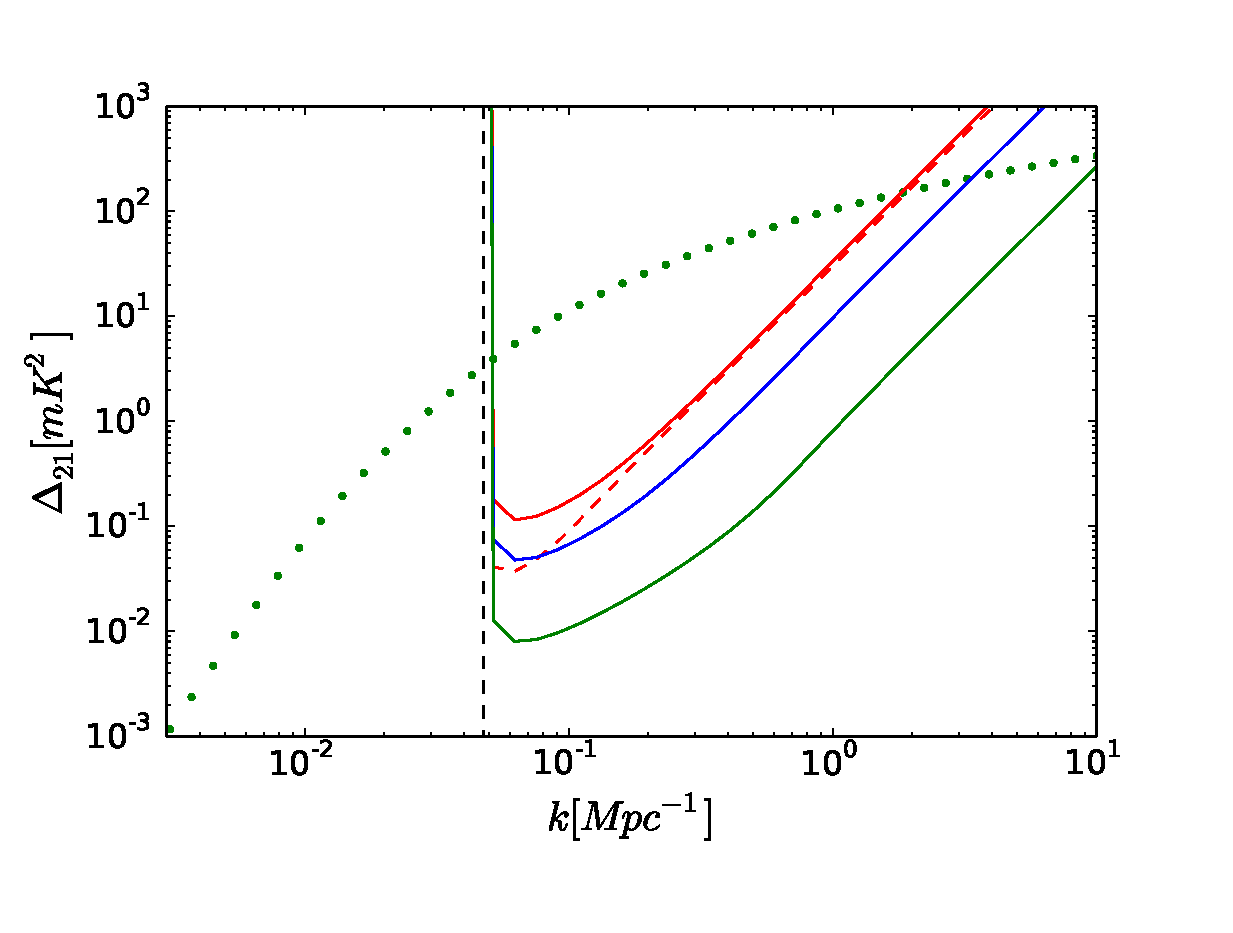
\includegraphics[scale=0.35]{figures/sensitivityPlot_z8.eps}
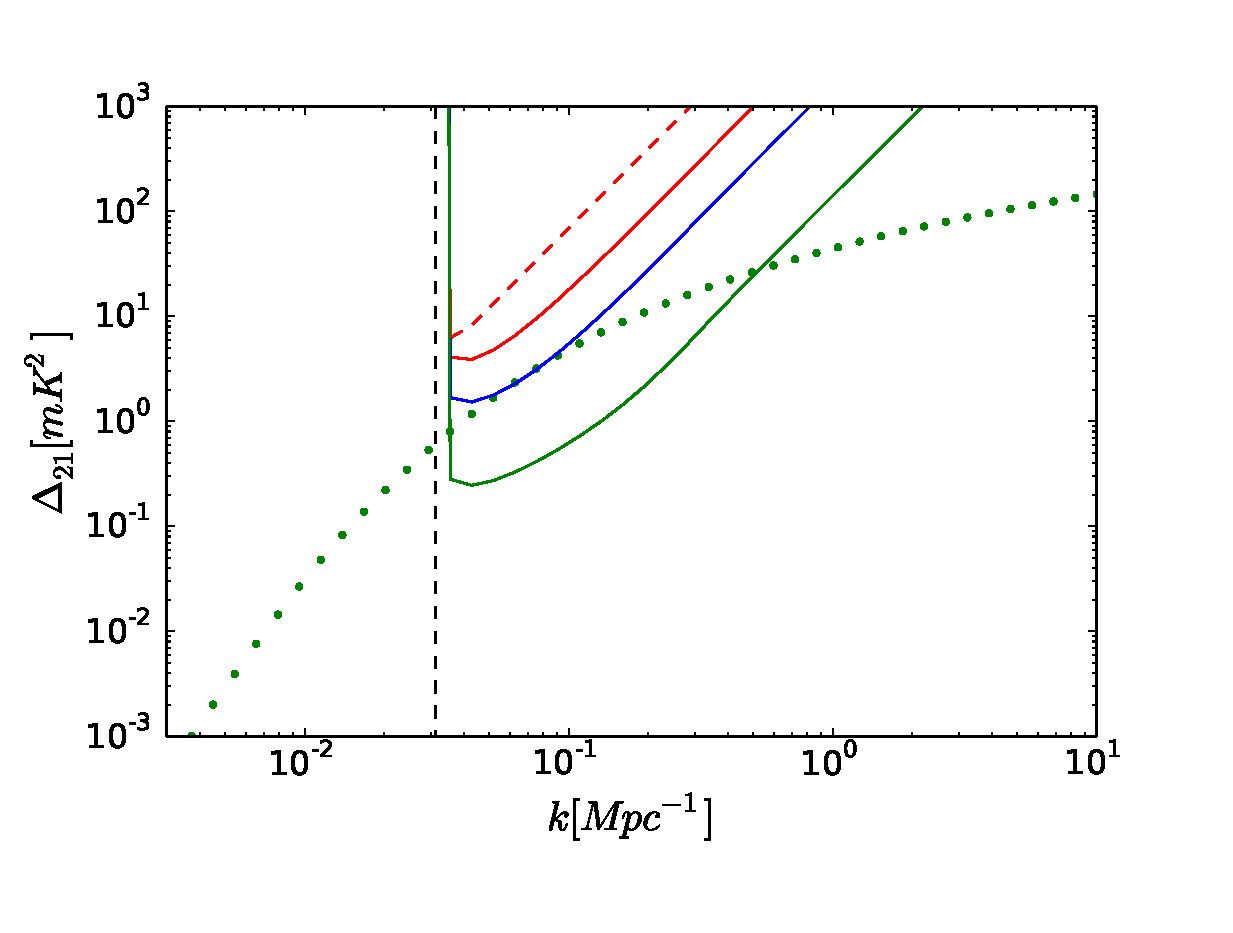
\includegraphics[scale=0.35]{figures/sensitivityPlot_z20.eps}
\caption{Sensitivity plots of HERA (red dashed curve), SKA0 (red), SKA1 (blue), and SKA2 (green). Dotted curve shows the predicted 21cm signal from the density field alone assuming $x_H=1$ and $T_S\gg T_{\rm CMB}$. Vertical black dashed line indicates the smallest wavenumber probed in the frequency direction $k=2\pi/y$, which may limit foreground removal.  {\em Left panel:} $z=8$ {\em Right panel:} $z=20$.}
\label{fig:sensitivity}
\end{center}
\end{figure}

Figure \ref{fig:sensitivity} illustrates a few key points governing parameter constraints. Here we have eliminated modes whose wavelength exceeds the instrument bandwidth removing sensitivity to the largest physical scales (smallest $k$ modes). At $z=8$, SKA0 is directly comparable in sensitivity to the proposed HERA experiment \cite{2014ApJ...782...66P}, which is more centrally concentrated to compensate for its small number of stations. By $z=20$ the amplitude of the 21 cm signal is too small to be detected by SKA1 {\em if we assume $T_S\gg T_\gamma$}. Detection of the 21cm signal at $z\gtrsim20$ with SKA1 is dependent upon a strong 21cm absorption signal that boosts the amplitude of the 21cm power spectrum. Unfortunately, it seems likely that during the absorption regime the details and spatial variation of the spin temperature will matter and complicated getting at cosmology.

The key parameters for determining cosmological parameters are the effective volume probed and the minimum wavenumber probed $k_{\rm min}$ where modes can still be assumed to be linear. SKA has a significant advantage over galaxy surveys as more modes are still in the linear regime at $z>6$. We set $k_{\rm min}=2{\rm Mpc^{-1}}$ at $z=8$ corresponding to the scale where $\sigma(2\pi/k)=0.5$.

\begin{figure}[htbp]
\begin{center}

\caption{Effective volume and comparison of SKA-LOW to Euclid}
\label{fig:effectivevolume}
\end{center}
\end{figure}

Comment on higher redshift giving other advantages, eg isocurvature, where effects become smaller deeper into matter dominated regime.

Table \ref{tab:constraints} shows the cosmological parameters obtained with the listed experimental performances.

\begin{table*}[htdp]
\caption{Fiducial parameter values and $1-\sigma$ experimental uncertainties for cosmological parameters.  Dashes indicate parameters not relevant for that experiment; $\infty$ indicates parameters that are relevant, but not constrained. }
\begin{center}
\begin{tabular}{c|cccccccc|c}
\hline
& $\Omega_mh^2$ & $\Omega_bh^2$ & $\Omega_\Lambda$ & $w$ & $n_s$ & $A^2_s$ & $\tau$ & $Y_{He}$  & $M_\nu$ \\
\hline
Fiducial& 0.147 & 0.023 & 0.7 & -1 & 0.95 & 26.6 & 0.1 & 0.24 & 0.3  \\
\hline
Planck & - & - & - & - & - & - & - & - & -   \\
HERA & - & - & - & - & - & - & - & - & -  \\
SKA0 & - & - & - & - & - & - & - & - & -  \\
SKA1 & - & - & - & - & - & - & - & - & -  \\
SKA2 & - & - & - & - & - & - & - & - & -  \\
\end{tabular}
\end{center}
\label{tab:constraints}
\end{table*}

\subsection{Core cosmological parameters}

\subsection{Inflationary parameters}

\subsection{Neutrino mass}



%%%%%%%%%%%%%%%%%%%%%%%%%%%%%
%%%%%%%%%%%%%%%%%%%%%%%%%%%%%
\section{Constraining new physics from heating}

The 21cm signal probes both the ionization and thermal state of the IGM.  Although we do not know the precise timing and evolution of the signal, empirical scaling relations based on local star-forming galaxies (e.g. Mineo+2012) suggest that the X-rays from early galaxies heat the IGM to temperatures above the CMB before the bulk of reionization (e.g. Furlaneto 2006; \S 2.1 in McQuinn \& O�Leary 2012).  This marks the transition of the 21cm signal from absorption to emission, with large-scale fluctuations in gas temperature likely driving the 21cm power to its largest amplitude (e.g. Pritchard \& Furlanetto 2007; Baek+2010).  The epoch of IGM heating is a powerful probe of the high-energy processes in the early Universe, with could have both astrophysical and cosmological origins.  Both can tells us about the nature of dark matter (DM).

In order to explain the apparent deficiencies of CDM on small (sub-Mpc) scales, Warm Dark Matter (WDM) models have recently gained in popularity.  In these models, DM is assumed to consist of smaller mass particles, $\sim$ keV, such as the sterile neutrino or gravitino.  The increased particle free-streaming and velocity dispersion (acting as a sort of effective pressure), can dramatically suppress structures on small-scales.  This suppression is even more obvious in the early Universe, where typical halos hosting galaxies were much smaller, and larger structures did not have time to fragment.  Current astrophysical lower limits on the WDM particle range from $m_x \gtrsim$ 1�3 keV (assuming a thermal relic relativistic at decoupling), with various degrees of astrophysical degeneracy (e.g. \cite{deSouza2013,Kang,Pacucci,Viel})

The resulting dearth of galaxies in the early Universe means that the astrophysical epochs in the 21cm signal were delayed.  The challenge as always will be to disentangle the cosmological impact from astrophysical uncertainties, such an a lower than expected star formation efficiency in CDM.  Since the fractional suppression of structure increases with redshift, this becomes much easier with the first galaxies observable with the SKA.  For example, we only need to understand the astrophysics of the first galaxies to an order of magnitude in order to improve on current $m_X$ constraints (Sitwell+
http://adsabs.harvard.edu/abs/2014MNRAS.438.2664S)
Moreover, even if the star-formation efficiency in CDM is allowed to vary in order to mimic the mean 21cm evolution in WDM models, the signal will still not be completely degenerate (see Fig. \ref{fig:darkmatter}a).  This is due to the fact that the galaxies driving the 21cm evolution in WDM should reside in higher mass, more rapidly evolving halos, than those in CDM.  The increased bias of such halos results in a larger 21cm fluctuations (see Fig. \ref{fig:darkmatter}a).

The heating of the IGM could also have a cosmological component.  In particular, annihilations of dark matter particles in the $\sim$ 10 GeV mass range (motivated by recent results from indirect experiments; e.g. \cite{Adriani, Abdo,Aguilar})
could provide a dominant source of heat, before the birth of the first galaxies.  Driven by the evolution of $\sim M_\cdot$ structures, several order os magnitude smaller than those hosting galaxies, heating is expected to be much slower in such models, resulting in a smaller brightness temperature gradient  $d\delta Tb/d? \sim4 mK MHz^{-1}$ in the range $? \sim 60 ? 80$ MHz (valdes+2013).  Moreover, DM annihilations would heat the IGM quite uniformly, which is not the case for heating driven by astrophysical sources residing in early galaxies.  The resulting lack of temperature fluctuations (see Fig. \ref{fig:darkmatter}b) would result in dramatic drop in 21cm power during heating, which would be easy to identify with the SKA (Evoli+ in prep).  Furthermore, the ensuing rise in 21cm power when the galaxies start contributing to heating the IGM should occur {\em when the IGM is already in emission}.  The later is a qualitatively robust signature of DM annihilation heating, easily obtainable with the SKA.



\begin{figure}[htbp]
\begin{center}
\includegraphics[scale=0.4]{figures/THist.eps}
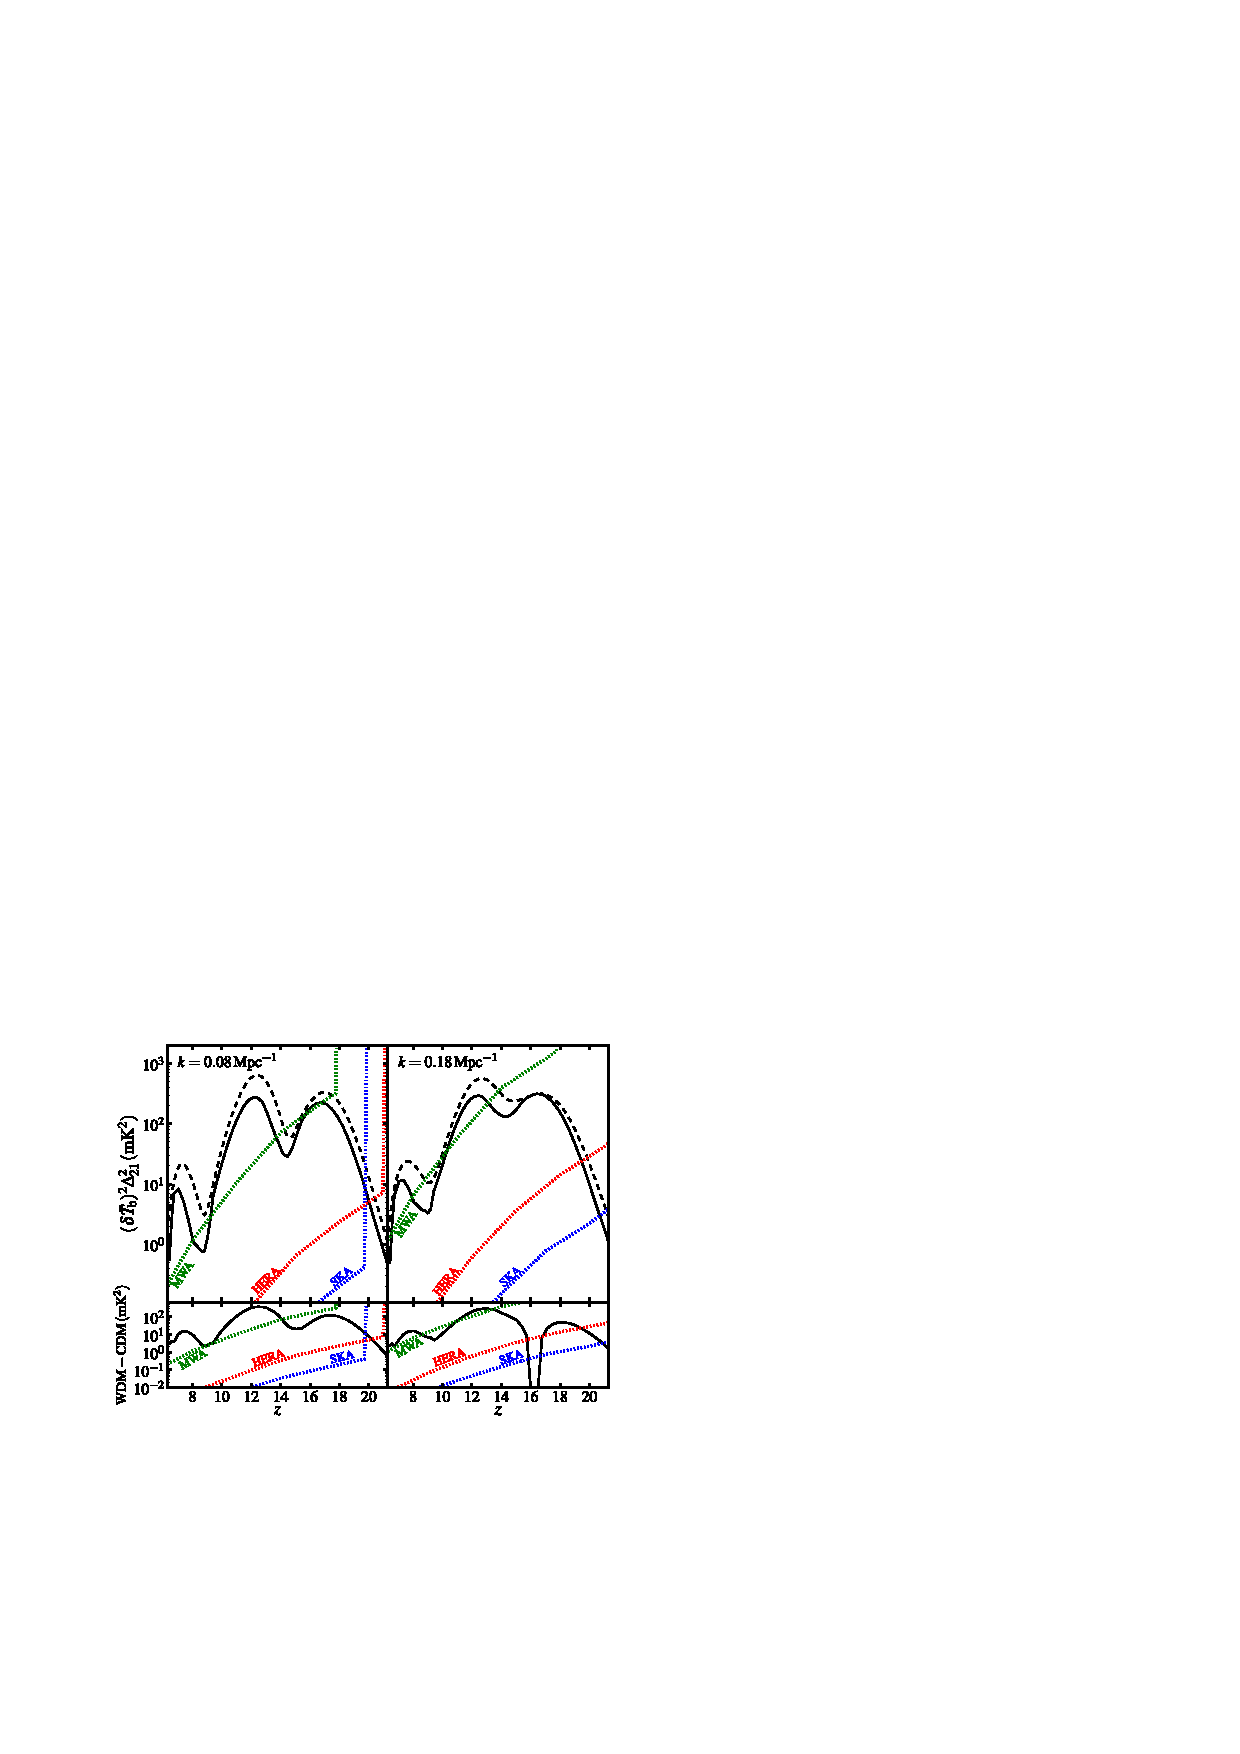
\includegraphics[scale=0.8]{figures/WDM_ps.pdf}
\caption{{\em Right panel: }Evolution of the power spectrum of ?Tb for WDM with $m_X = 2$ keV. The top panels show power spectra at
k = 0.08, 0.18 Mpc?1 for WDM (dashed) and the CDM model (solid). CDM models have f?(z) (star-formation efficiency) chosen to reproduce the global 21-cm signal found for
the respective WDM model. The bottom panels show the difference in the power spectrum between WDM and CDM models. Dotted curves show forecasts
for the 1? power spectrum thermal noise as computed in Mesinger et al. (2013a) assuming 2000 h of observation time. The dotted green, blue and red curves are
the forecasts for the MWA, SKA and HERA, respectively.  This figure is from Sitwell+2014.
CDFs of T?/TS corresponding to the fiducial and extreme astrophysical X-ray heating (black and gray curves respectively) from Mesinger+2013.  The colored curves correspond to models in which 10 GeV DM annihilations are also accounted for (in addition to fiducial astrophysical heating), with varying relative contribution. The curves correspond to the redshift for which Ts ? TCMB. Figure is from Evoli, mesinger, Ferrara, in prep.}
\label{fig:darkmatter}
\end{center}
\end{figure}

%%%%%%%%%%%%%%%%%%%%%%%%%%%%
% Magnetic fields
%%%%%%%%%%%%%%%%%%%%%%%%%%%%
\subsection{21 cm signal from the PMFs}

Primordial magnetic fields (PMFs) has been intensively investigated in
the literature as possible seeds for large scale magnetic fields
observed in galaxies and clusters of galaxies (for a recent review, see
\cite{2013A&ARv..21...62D}).  Magnetic fields in galaxies in high
redshifts \cite{2008Natur.454..302B} and in void regions
\cite{2010Sci...328...73N,2010ApJ...722L..39A,2013ApJ...771L..42T} can
well be the pieces of evidence that the seed fields are of primordial
origin.  The primordial magnetic fields may be created in the very
early universe, e.g., at the epoch of inflation, cosmological phase
transition, and cosmological recombination.  
The Planck collaboration
recently places limits on the PMFs as $B_{\lambda=1{\rm Mpc}} < 3.4$ nG and $n_B<0$
from the temperature anisotropies on large and small angular scales
\cite{2013arXiv1303.5076P}. 

The CMB brightness temperature fluctuations produced by the neutral
hydrogen 21-cm line (21 cm) would offer a new probe of the primordial
magnetic fields (PMFs) created in the early universe. For the 21 cm
observation, aside from the early structure formation effect by the
Lorentz force from the PMFs, one of the important effects is the
dissipation process of the PMFs that increases the baryon
temperature. The dissipation occurs mainly through the ambipolar
diffusion due to the velocity difference between neutral hydrogen (which
is the dominant component in the dark ages) and ionized particles (whose
trajectory is bent by the Lorentz force).  The effect of the dissipation
is rather significant. The gas temperature can reach $1000$ K or even
$10^4$ K at $z=30$ if the magnetic fields have the strength of
$B_\lambda \sim 3$ nG
\cite{2005MNRAS.356..778S,2006MNRAS.372.1060T,2009ApJ...692..236S,2014JCAP...01..009K}.

This dissipation will give rise to a unique signature of the PMFs on the
21 cm observation. Because the spin temperature is closely coupled to
the gas temperature at high redshift ($z>30$), the 21 cm signal would
come as `emission' if the energy dissipation is efficient. In
Fig.~\ref{fig:KI1} the global HI signal with several magnetic field
strengths are shown. For cases with sufficient magnetic fields, say
$B\gtrsim 0.03$ nG, the signal is always emission against CMB while in
the standard $\Lambda$CDM model the signal would be absorption for the
frequency range of $f_\nu \lesssim 80$ MHz (corresponding to the signal
from redshift $z\gtrsim 20$).
\begin{figure}[]
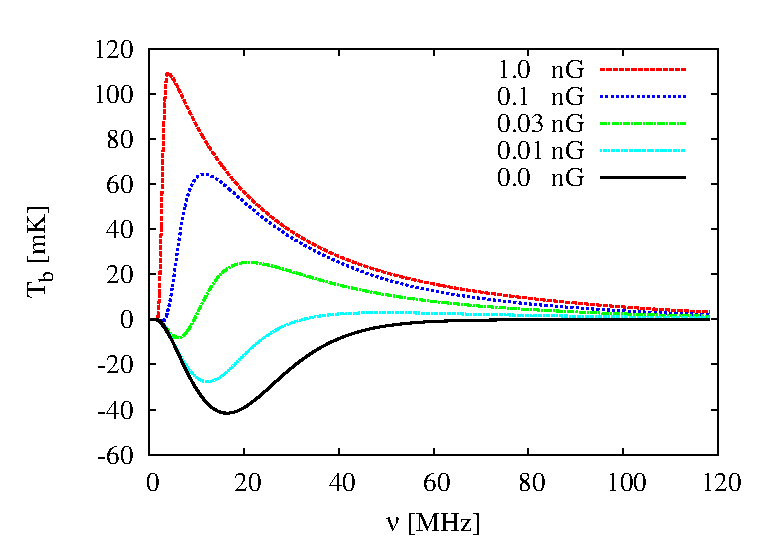
\includegraphics[width=0.5\linewidth,angle=0]{figures/KI_fig1.eps}
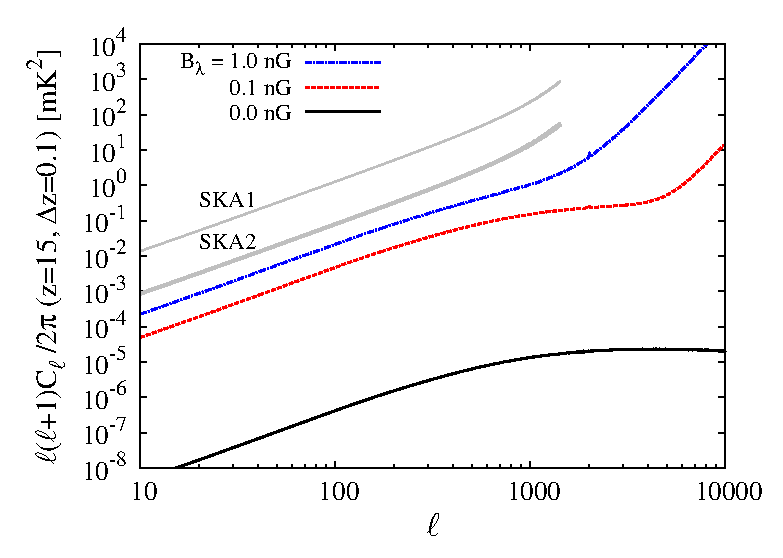
\includegraphics[width=0.5\linewidth,angle=0]{figures/KI_fig2.eps}
\caption{{\em Left panel: }The global 21 cm signal with magnetic field strength $B=1$
$0.1$, $0.03$, and $0.01$ nG (colored lines from top to bottom). The
solid line corresponds to the model without primordial magnetic fields.
Note that any other heating source than magnetic fields is neglected in
the figure. {\em Right panel: }Angular power spectra for PMF strengths: $B=0,~ 0.1,~ 1.0$ nG
at $z=15$. The bottom curve shows the power spectrum from the standard
density perturbations for fully neutral medium without any heating and
reionization processes. The red and blue curves correspond to the cases
with heating by the PMFs with $B=0.1$ nG and $B=1.0$ nG,
respectively. The heating induces deviations of the spin temperature
from the CMB temperature and the signal is enhanced. The noise curves
for SKA1 and SKA2 are also shown as indicated. By courtesy of
M. Shiraishi \& H. Tashiro.}  \label{fig:KI1}
\end{figure}

We show the angular power spectrum of the 21 cm brightness temperature
including the PMFs in Fig.~\ref{fig:KI1}b
\cite{2014arXiv1403.2608S}. Here we do not account for any (standard)
heating effects (i.e., UV, X, and L$\alpha$ background emissions) to isolate and
clarify the effects from the PMFs.  On large scales which may be
relevant to SKA 
observations, there are two distinct contributions. One is from the
standard (adiabatic) density fluctuations enhanced by the heating from
the PMFs, and the other is from the PMF induced density fluctuations
dominant on smaller scales
\cite{2006MNRAS.372.1060T,2009ApJ...692..236S}. We can see from the
figure that $B=1$ nG
magnetic fields are marginally within reach for a statistical detection
of the power spectrum. Stacking observing channels in principle will add
more statistical power.

The angular correlation function in real space including the effects
from the PMFs is also studied in \cite{2009JCAP...11..021S}.  The
function exhibits a distinct feature because the PMFs induce early
structure formation and the small scale halos form more compared to the
case in the standard $\Lambda$CDM model The signal from primordial
magnetic fields shows oscillatory feature contrary to that in the
standard $\Lambda$CDM since the matter power spectrum induced by the
PMFs is blue and most of halos are formed at the scale close to the
magnetic Jeans' length. It has been argued that $5$ sigma detection of
the $0.5$ nG magnetic fields will be possible with less than one week
integration of SKA observation \cite{2009JCAP...11..021S}.



%%%%%%%%%%%%%%%%%%%%%%%%%%%%%
%%%%%%%%%%%%%%%%%%%%%%%%%%%%%
\section{Fundamental physics from modifications to the source population}

Non-Gaussianity from bispectrum and power spectrum as a result of modification to source populations.

%%%%%%%%%%%%%%%%%%%%%%%%%%%%%
%%%%%%%%%%%%%%%%%%%%%%%%%%%%%
\section{Bulk flows}

BAO and consistency from signal during relative velocity flow epoch.

%%%%%%%%%%%%%%%%%%%%%%%%%%%%%
%%%%%%%%%%%%%%%%%%%%%%%%%%%%%
\section{Cosmic shear and the EoR}
It is possible that the EoR signal could be used to measure weak gravitational lensing.
In \cite{Zahn:2005ap} and \cite{Metcalf:2009}  it was shown that if the EoR is at redshift 
$z \sim 8$ or later, a large radio telescope such as the SKA could measure the lensing convergence power spectrum.  However a very large $f_{\rm sky}$ and a very compact low frequency array was assumed by those authors.  Here the calculation is repeated with parameters that are more consistent with current SKA plans.  The current plans for a 25 square degree survey with SKA\_Low will preclude measuring cosmological parameters through their effects on the weak lensing power-spectrum because of large sample variance.  (This is not true of the SKA\_Mid at lower redshift where the survey area will be much larger. See section *** for more details.)  It still might be possible to map the lensing convergence within the 25 square degree EoR survey area.  This would allow us to actually ``see'' the distribution of dark matter in a typical region of the sky, something that is only possible with galaxy lensing around very atypical, large galaxy clusters.  This would provide a great opportunity to correlate visible objects with mass and test the dark matter paradigm.

The previously mentioned authors extended the
Fourier-space quadratic estimator technique, which was first developed in 
\cite{Hu:2001tn} for CMB lensing  observations to three dimensional
observables, i.e. the $21$ cm intensity field $I(\theta,z)$.  
The  convergence
estimator and the corresponding lensing reconstruction noise are
calculated assuming that the temperature (brightness) distribution is
Gaussian. This will not be strictly true during the EoR, but serves as a reasonable approximation for these purposes. Note that the lensing reconstruction noise contains the thermal noise of the telescope which is calculated using the formula
\begin{equation}
C^{\rm N}_\ell = \frac{(2\pi)^3 T^2_{\rm sys}}{B t_{\rm obs} f^2_{\rm cover} \ell_{\rm max}(\nu)^2} \, ,
\end{equation} where the system temperature $T_{\rm sys}$ at high redshifts
 is dominated by galactic synchrotron radiation, $B$ is the chosen frequency window, $t_{\rm obs}$ the total observation time, $D_{\rm tel}$ the diameter (maximum baseline) of the core array, $\ell_{\rm max}(\lambda)=2\pi D_{\rm tel}/\lambda$ is the highest multipole that can be measured by the array at frequency $\nu$ (wavelength $\lambda$), and $f_{\rm cover}$ is the total collecting area of the core array $A_{\rm coll}$ divided by $\pi(D_{\rm tel}/2)^2$. 
 
 The advantage of 21cm lensing is that one is able to combine
information from multiple redshift slices. In Fourier space, the
temperature fluctuations are divided into perpendicular to the line of
sight wave vectors $\mathbf{k_\perp}=\mathbf{l}/r$, with $r$ the angular diameter distance to the source redshift, and a
discretized version of the parallel wave vector $k_\parallel =
\frac{2\pi}{{\cal L}}j$, where ${\cal L}$ is the depth of the observed
volume. Considering modes with different $j$ independent, an optimal
estimator can be found by combining the individual estimators for
different $j$ modes without mixing them. The three-dimensional lensing reconstruction noise is then found to be  \cite{Zahn:2005ap}\begin{equation}
N(L,\nu) =  \left[\sum_{j=1}^{j_{\rm max}} \frac{1}{L^4}\int \frac{d^2\ell}{(2\pi)^2}  \frac{[\mathbf{l} \cdot \mathbf{L} C_{\ell,j}+\mathbf{L} \cdot (\mathbf{L}-\mathbf{l})
C_{|\ell-L|,j}]^2}{2 C^{\rm tot}_{\ell,j}C^{\rm tot}_{|\mathbf{l}-\mathbf{L}|,j}}\right]^{-1}.
\end{equation}
Here, $C^{\rm tot}_{\ell,j}=C_{\ell,j}+C^{\rm N}_\ell$, where $C_{\ell,j}=[\bar{T}(z)]^2P_{\ell,j}$ with $\bar{T}(z)$ the mean observed brightness temperature at redshift $z$ due to the average HI density and $P_{\ell,j}$ the underlying dark matter power spectrum  \cite{Zahn:2005ap}. 
For SKA\_Low we can consider a $1,000~{\rm hr}$ observation time and we choose $B = 8 \, {\rm MHz}$ and $j_{\rm max}=40$, but with multiple bands $\nu$ that can be stacked to reduce the noise so that $N_L = 1/\displaystyle\sum_{\nu} [N(L,\nu)]^{-1}$. 
 
At redshift $z_s \sim 8$, we can assume the SKA1 Baseline Design \cite{Dewdney:2013} parameters of $A_{\rm coll} \simeq 0.3  \, {\rm km}^2$ with maximum baseline $D_{\rm tel}=4 \, {\rm km}$, while for SKA2 we can consider $A_{\rm coll} \simeq 1.2  \, {\rm km}^2$.
The estimated lensing noise is shown in Figure~\ref{fig:CLNL} along with the estimated signal.  
Here $C_L$ is the convergence field power spectrum at $z_s=8$ and $N_L$ the lensing reconstruction noise assuming a reionization fraction $f_{\rm HI}=1$.
\begin{figure}[h]
\centerline{
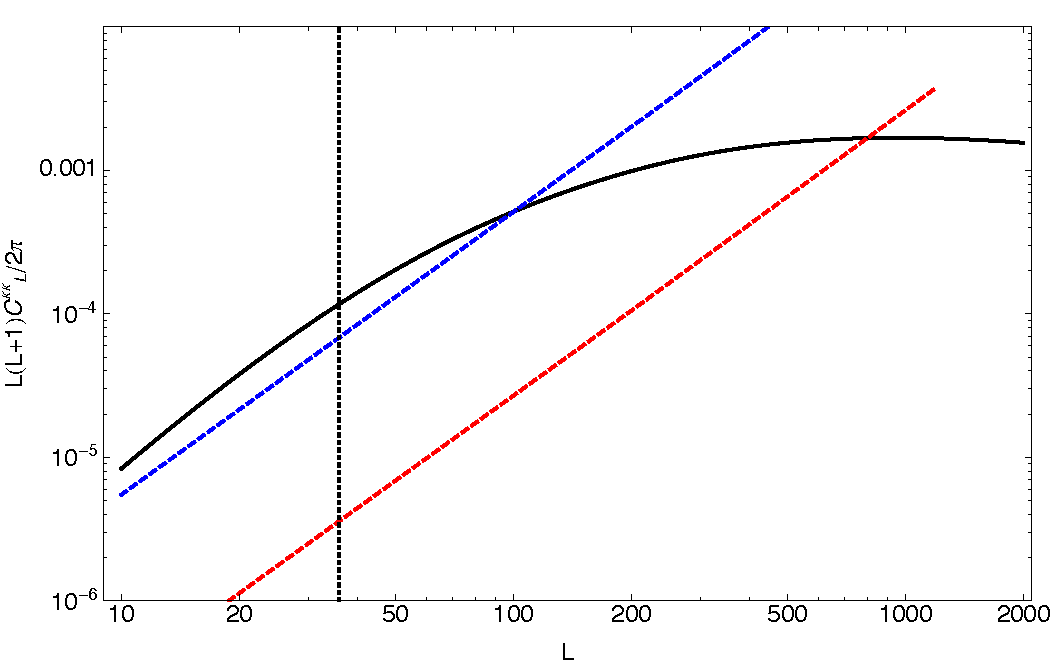
\includegraphics[scale=0.5]{figures/tomographic_SKA_kappaPS.pdf}
}
\caption{The lensing convergence field power spectrum, $C_L$, for sources at $z=8$ is shown as a solid black line and lensing reconstruction noise $N_L$ as dashed lines.  The blue dashed curve is for the SKA1 Baseline Design with 10 8~MHz frequency bins around $z=8$ spanning the redshift range $z \simeq 6.5-11$.  The red line is for SKA2 and the same frequency bins. The vertical line is approximately the lowest $L$ accessible with a 5-by-5 degree field.  Where the noise curves are below $C_L$, typical fluctuations in the lensing deflection should be recoverable in a map. }
\label{fig:CLNL}
\end{figure}

These results show that it might be possible to map the lensing signal over a range of angular scales.  This measurement greatly benefits from the larger collecting area that will come with Phase 2 of the SKA (we also note that  considering a more compact array, i.e. smaller $D_{\rm tel}$, also improves the signal-to-noise).  The weak lensing power spectrum can be better measured for redshifts after reionization using SKA\_Mid and the same 21 cm intensity mapping technique discussed, but over a much larger area of sky \cite{PourtsidouMetcalf:2014}.

%%%%%%%%%%%%%%%%%%%%%%%%%%%%%
%%%%%%%%%%%%%%%%%%%%%%%%%%%%%
\section{Separating ``gastrophysics" and cosmology}
\label{sec:separation}

The key challenge for extracting fundamental physics from the 21cm signal will be separating the effects of cosmology from ``gastrophysics". A number of avenues have been studied in the literature, which broadly separate into (1) avoidance and (2) modelling. In the absence of a clearly defined window where $T_S\gg T_{\rm CMB}$ and $x_H=1$ it might still be possible to avoid astrophysics via the angular dependence of the power spectrum induced by redshift space distortions. Focussing on the $P_{\mu^4}\approx P_\delta$ part could lead to clean cosmological measurements. Obtaining precision cosmology this way is hard and the literature suggests little improvement over Planck is possible \cite{2006ApJ...653..815M,2008PhRvD..78b3529M}. Figure \ref{fig:musensitivity} shows predicted errors bars for SKA1 on the $P_{\mu^2}$ and $P_{\mu^4}$ parts of the power spectrum. A detection is possible with reasonable sensitivity at wavenumbers $k=0.1-1{\rm\,Mpc^{-1}}$.

\begin{figure}[htbp]
\begin{center}
\includegraphics[scale=0.35]{figures/musensitivityPlot_z8.eps}
\caption{Sensitivity plots on $P_{\mu^2}$ and $P_{\mu^4}$ for HERA (red dashed curve), SKA0 (red), SKA1 (blue), and SKA2 (green). Dotted curve shows the predicted 21cm signal from the density field alone assuming $x_H=1$ and $T_S\gg T_{\rm CMB}$. Vertical black dashed line indicates the smallest wavenumber probed in the frequency direction $k=2\pi/y$, which may limit foreground removal.  {\em Left panel:} $z=8$ {\em Right panel:} $z=20$.}
\label{fig:musensitivity}
\end{center}
\end{figure}

Information in $P_{\mu^2}$ is likely to help with modelling of the astrophysics. 

Compared with the CMB our theoretical understanding of the 21cm signal during reionization is poor. Predictions for the 21cm power spectrum do not exist at the same level of precision as the cosmology. Nonetheless, we expect the contribution of astrophysics to be relatively broad band and determined by extra power about a characteristic scale, eg the bubble size during reionization.

%%%%%%%%%%%%%%%%%%%%%%%%%%%%%
%%%%%%%%%%%%%%%%%%%%%%%%%%%%%
\section{Paths to cosmology with Phase 1 and Phase 2}

Short section to comment on what Phase 2 gets you over Phase 1.

%%%%%%%%%%%%%%%%%%%%%%%%%%%%%
%%%%%%%%%%%%%%%%%%%%%%%%%%%%%
\section{Miscellaneous?}

Other ways of constraining cosmology unique to SKA: variation of fine structure, cosmic string wakes, etc


%%%%%%%%%%%%%%%%%%%%%%%%%%%%%
%%%%%%%%%%%%%%%%%%%%%%%%%%%%%

%JRP use bibtex while editing
\bibliographystyle{unsrt}
\bibliography{cosmchapterbib}{}
%%% END JRP

%%% Fill copy in .bbl at end
%\begin{thebibliography}{99}
%\bibitem{...}
%\end{thebibliography}
% END COMMENTED OUT BIB

\end{document}
